\documentclass[aspectratio=169]{beamer}
\usetheme{default}
\usepackage{booktabs}
\usepackage{graphicx}
\definecolor{editblue}{RGB}{38,117,168}
\setbeamercolor{structure}{fg=editblue}
\title{Is the sequence editor sensitive to learning rate?}
\subtitle{Separating optimization effects from random variation}
\date{18 July 2026}
\begin{document}
\frame{\titlepage}

\begin{frame}{The question is about fair comparisons}
  \begin{itemize}
    \item The learning rate controls how far the model moves after each training signal.
    \item Too small a rate can make a healthy model look weak simply because training ends too soon.
    \item Random seeds cause a different problem: initialization and example order vary between otherwise identical runs.
    \item We need to measure both before attributing a score change to a new architecture or objective.
  \end{itemize}
  \vfill
  \textbf{Why it matters:} width, counterfactual losses, LDAD, GAR, and hierarchy may each prefer different update sizes.
\end{frame}

\begin{frame}{Only the peak learning rate changes}
  \begin{itemize}
    \item Every cell uses fixed mixed corruptions, token-aligned EMA targets, K=0, d256, batch eight, and no dropout.
    \item Training contains 6,000 unique iGSM problems over three epochs, or 18,000 presentations.
    \item The sweep spans $10^{-6}$ through $3\times10^{-4}$ under the same cosine schedule.
    \item Nine new seed-zero cells are combined with the existing three-seed endpoint at $3\times10^{-4}$.
    \item Each completed checkpoint is evaluated on 256 held-out mixed-edit examples.
  \end{itemize}
  \vfill
  \textbf{What to notice:} this isolates optimization sensitivity for the current primitive, not for every future method.
\end{frame}

\begin{frame}{Performance improves smoothly across the requested range}
  \centering
  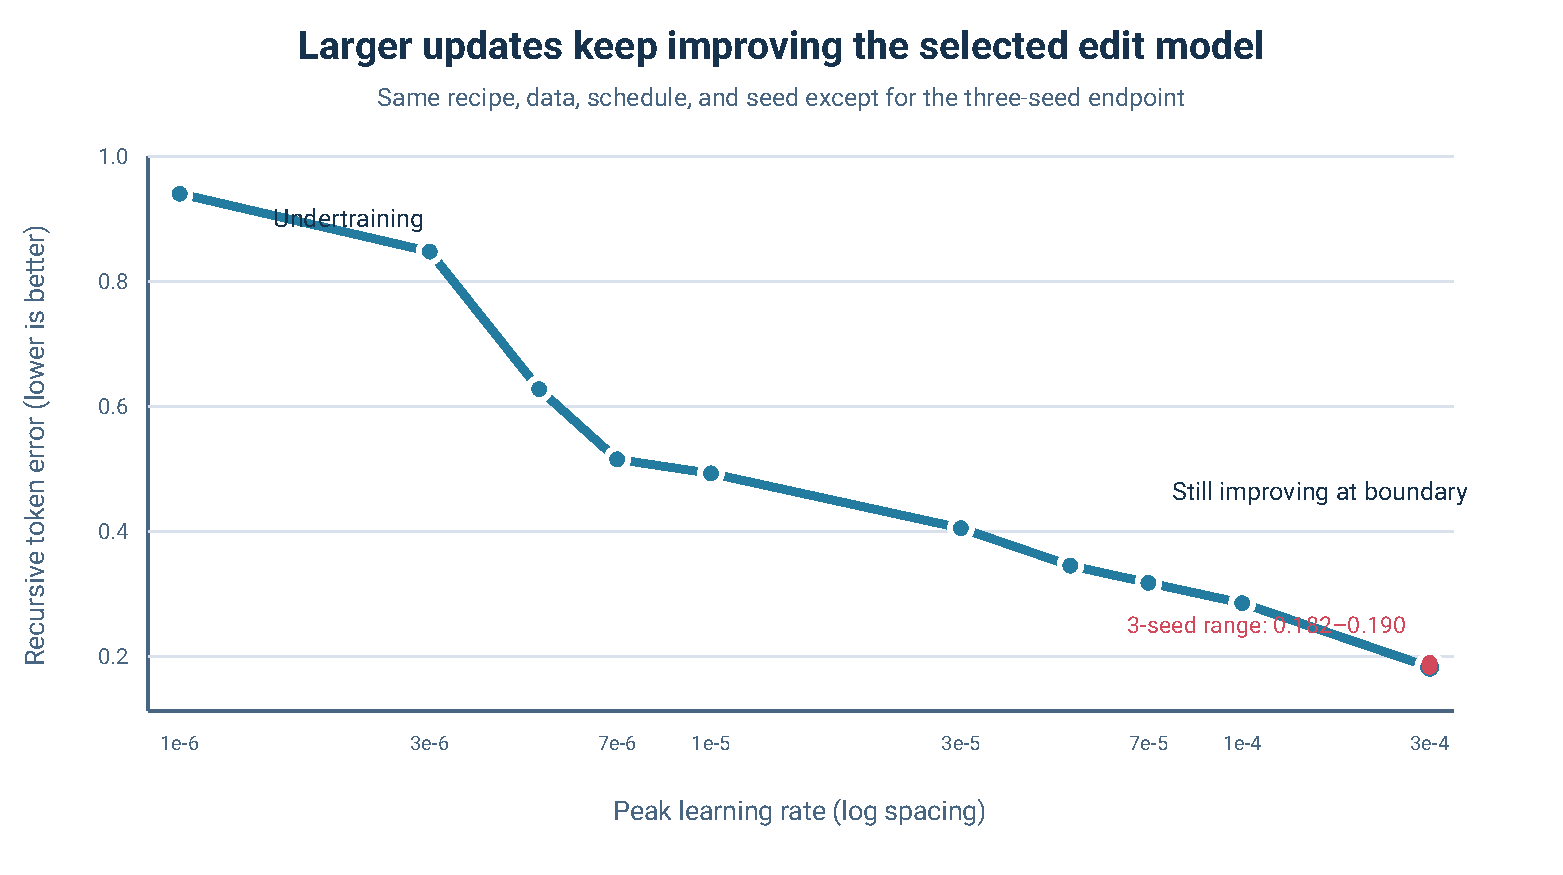
\includegraphics[width=0.91\textwidth]{lr_curve.pdf}
\end{frame}

\begin{frame}{Learning-rate effects dwarf seed noise}
  \centering
  \begin{tabular}{lrrr}
    \toprule
    Condition & Matched error & Recursive error & Action ratio \\
    \midrule
    $10^{-6}$ & .916 & .941 & 1.04 \\
    $10^{-5}$ & .411 & .492 & 1.76 \\
    $10^{-4}$ & .169 & .285 & 3.31 \\
    $3\times10^{-4}$, seed 0 & .095 & .182 & 5.22 \\
    $3\times10^{-4}$, seeds 1/2 & .100/.096 & .190/.185 & 5.02/5.22 \\
    \bottomrule
  \end{tabular}
  \vfill
  \begin{itemize}
    \item Moving from $10^{-4}$ to $3\times10^{-4}$ cuts recursive error by about 36\%.
    \item The full seed range at $3\times10^{-4}$ is only about 4.3\%.
    \item Gradient norms remain benign, so low rates undertrain rather than explode.
  \end{itemize}
\end{frame}

\begin{frame}{The evidence changes how methods must be compared}
  \begin{itemize}
    \item The large exposure and width gains remain larger than measured seed noise, but width needs its own learning-rate cross-check.
    \item K=1's 3--4\% recursive penalty is comparable to seed spread and must be retested across rate and loss weight.
    \item LDAD and GAR alter loss scale, so a common untuned rate would be especially unfair to them.
    \item Identical fixed-versus-fresh corruption results remain strong because those cells share the same parameterization and objective.
  \end{itemize}
  \vfill
  \textbf{Why it matters:} systematic optimization sensitivity is a confound, but it is not random fluctuation.
\end{frame}

\begin{frame}{Next, bracket the optimum before adding complexity}
  \begin{itemize}
    \item Reuse $3\times10^{-4}$ and test $2\times10^{-4}$, $5\times10^{-4}$, $7\times10^{-4}$, and $10^{-3}$ until the curve turns over.
    \item Confirm the selected primitive rate with at least three seeds.
    \item Give d512 and K=1 separate three-point learning-rate controls; cross K=1 with weights 0.25 and 1.
    \item Tune GAR H1/H4 only after the primitive is fixed, then compare hierarchy against a separately tuned flat control.
    \item Attempt MPC, beam search, or CEM only after recursive dynamics and GAR ranking pass their gates.
  \end{itemize}
\end{frame}
\end{document}
